\documentclass[main.tex]{subfiles}
\begin{document}
\textbf{Exercise 1. Fermat's Principle}\\
Lifeguard Alice can run at speed $v_r$ on the beach and swim at speed $v_s$ in the water, with $v_r > v_s$. What is the path that minimizes the time for reaching point B and saving Bob from drowning?


\begin{figure}
\centering\fbox{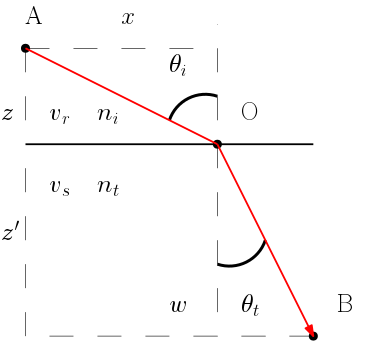
\includegraphics[height=2.0in]{figures/hw1_1.png}}
\caption{Path traveled by Alice \textbf{A} to reach Bob \textbf{B} which minimizes travel time.}
\label{fig:1}
\end{figure}

\textbf{Answer}\\
$\because v_r > v_s$ and \\
$\because$ Snell's law states the relationship between the incident index and angle and the transmission index and angle is defined as: $n_i\sin(\theta_i) = n_t \sin(\theta_{t})$ and\\
$\because$ velocity of light and material index are inversely related as follows:  $n_i = c / v_r$ and $n_t = x / v_s$ and \\
$\because$ the Path the light  (aka lifeguard Alice), shown in Figure \ref{fig:1},  travels  = $AO + OB = n_i \sqrt{(x^2 + z^2)} + n_t \sqrt{(w-x)^2 +  z^{\prime 2}}$ and\\
$\because$ the Shortest Path is determined by setting the derivative equal to zero such that $ \frac{\partial \text{Path}}{\partial x} = n_i \frac{x}{\sqrt{(x^2 + z^2)}} - n_t \frac{w-x}{\sqrt{((w-x)^2 + z^{2\prime 2})}} = 0$ and by substituting for velocity and simplifying we arrive at\\
$\frac{1}{v_r} \frac{x}{\sqrt{(x^2 + z^2)}} = \frac{1}{v_s} \frac{w-x}{\sqrt{((w-x)^2 + z^{2\prime 2})}} $ \\




\end{document}
